\documentclass[10pt]{article}
\usepackage[utf8]{inputenc}
\usepackage[T1]{fontenc}
\usepackage{geometry}
\geometry{a4paper, margin=0.75in}

% --- Math Packages ---
\usepackage{amsmath, amssymb, amsthm}

% --- Image Packages ---
\usepackage{graphicx}
\usepackage{float} % For forcing figure placement with [H]

% --- Table Packages ---
\usepackage{booktabs} % For professional looking tables
\usepackage{multirow}
\usepackage{longtable}

% --- Code Formatting ---
\usepackage{listings}
\usepackage{xcolor}

\lstset{
    basicstyle=\ttfamily\small,
    keywordstyle=\color{blue},
    stringstyle=\color{red},
    commentstyle=\color{green!60!black},
    numbers=left,
    numberstyle=\tiny\color{gray},
    stepnumber=1,
    breaklines=true,
    frame=single,
    showstringspaces=false
}

% --- Algorithm Packages ---
\usepackage{algorithm}
\usepackage{algpseudocode}

% --- Links and References ---
\usepackage{hyperref}
\hypersetup{
    colorlinks=true,
    linkcolor=blue,
    filecolor=magenta,
    urlcolor=cyan,
}

\title{Curve, Freeze, Thaw: HPO with FT-PFN}
\author{Yahya Fati Haji}
\date{\today}

\begin{document}
\maketitle

\section*{Problem Formulation}

Let $\Lambda$ be a hyperparameter search space and $f(\lambda, b)$ the performance (validation
accuracy, in this project) of configuration $\lambda \in \Lambda$ after being trained for $b$ discrete
training steps (epochs, here). A configuration's \textit{learning curve} is the sequence
$\{f(\lambda, 1), f(\lambda, 2), …\}$ as $b$ grows.

Freeze-thaw HPO relaxes the usual \textit{"pick a config, train it to completion, observe one
number"} protocol. Instead, resources are spent \textbf{incrementally}: at every iteration
the optimizer either \textbf{thaws} (resumes/continues) a previously partially-trained,
currently-frozen configuration for one more step, or starts a brand-new configuration.

Formally, the goal is to find a resource allocation that maximizes

$$
\max_{\lambda \in \Lambda,\ 1 \le b \le b_\lambda} f(\lambda, b)
$$
subject to
\begin{align*}
    N = |\{\text{decisions made}\}| \le B, \qquad
    b_\lambda^{\min} \le\  b_\lambda \le b_\lambda^{\max}, \\
    \forall\, \lambda \in \Lambda \ \text{with } b_\lambda > 0, \quad
    b_\lambda \in \mathbb{Z}_{\ge 0}, \quad
    \forall\, \lambda \in \Lambda
\end{align*}

\begin{itemize}
    \item a total trial budget, $B$ - the number of freeze/thaw decisions the optimizer is allowed to make.
    \item $b_\lambda^{\min}$ and $b_\lambda^{\max}$ - per-configuration epoch bounds that prevent premature judgments on too
little training and wasted spend on configs that have already converged.
\end{itemize}

\section*{The FT-PFN Surrogate}

Rather than fitting a Gaussian Process or random forest online (as SMAC/BOHB do), ifBO
uses \textbf{FT-PFN}, a \textit{Prior-data Fitted Network}: a transformer trained once, offline, on
large quantities of \textbf{synthetic} learning-curve data sampled from a hand-designed
prior, and then used purely for inference at HPO time via \textit{in-context learning} — no
weights are updated during the actual HPO run.

The implementation follows \textbf{ifBO} as introduced in:
\begin{quote}
H. Rakotoarison, S. Adriaensen, N. Mallik, S. Garibov, E. Bergman, F. Hutter.
\emph{In-Context Freeze-Thaw Bayesian Optimization for Hyperparameter Optimization.}
ICML 2024. \url{https://arxiv.org/abs/2404.16795}
\end{quote}

\subsection*{What the surrogate models}

FT-PFN approximates the posterior predictive distribution

\begin{equation}
p\big( f(\lambda_\text{test}, b_\text{test}) \mid \lambda_\text{test}, b_\text{test}, H \big)
\end{equation}

i.e., ``given everything observed so far about \emph{other} (and this) configurations'
partial learning curves, what is the distribution over this configuration's performance
at some future training step $b_\text{test}$?'' The set $H$ is passed to the network as a sequence
of tokens (its \textbf{context}) at inference time; the transformer's attention mechanism
implicitly performs Bayesian updating over this context in a single forward pass,
rather than through iterative model refitting. This is what makes each acquisition
query cheap enough to run every freeze-thaw step (the paper reports 10--100$\times$ speedups
over refitting-based gray-box surrogates such as DPL and DyHPO).

\section*{Acquisition function: MFPI and MFPI-random}

\subsection*{The paper's definition}

Multi-fidelity Probability of Improvement, as defined in the paper (Eq.\ 3):

\begin{equation}
\operatorname{MFPI}(\lambda; h, T) = P\big( M(\lambda, \min(b_\lambda + h, b_{\max})) > T \big)
\end{equation}

--- the surrogate-predicted probability that configuration $\lambda$, if thawed for $h$ more
steps, would exceed a target performance $T$. Two ``hyper-hyperparameters'' govern it: the
lookahead horizon $h$ and the improvement target $T$. Rather than fixing these, the paper
proposes \textbf{MFPI-random} (Eq.\ 4), redrawing both \textbf{every single freeze-thaw iteration}:

\begin{align}
\operatorname{MFPI\text{-}random}(\lambda) &= \operatorname{MFPI}(\lambda; h_\text{rand}, T_\text{rand}) \\
h_\text{rand}        &\sim U(1, b_{\max}) \\
T_\text{rand}        &= f_\text{best} + \tau_\text{rand} \cdot (1 - f_\text{best}) \\
\log_{10}(\tau_\text{rand}) &\sim U(-4, -1)
\end{align}

where $f_\text{best}$ is the best performance observed so far. This amounts to sampling an
acquisition function from an implicit \emph{portfolio} of MFPI instances at every step,
which the paper's ablations (Figure 4) show is necessary --- fixed-horizon or
fixed-threshold variants, and standard Expected Improvement paired with FT-PFN's
heavy-tailed posteriors, both underperform substantially.

\section*{Growing the candidate pool}

The paper's Algorithm 1 (see the pseudocode in the appendix of the original paper) is stated over the \emph{whole} search
space $\Lambda$ implicitly --- at each iteration the acquisition is (conceptually) maximized over
all $\lambda \in \Lambda$, which naturally lets brand-new, never-tried configurations compete against
partially-trained ones for being selected next.

This implementation instead maintains an \textbf{explicit, dynamically growing list} of candidates
(starting empty), and layers an \textbf{explicit decaying $\epsilon$-greedy exploration floor} on top
of MFPI-random rather than substituting for it:

\begin{align}
\epsilon(t) &= \epsilon_{\min} + (\epsilon_0 - \epsilon_{\min}) \cdot \left(1 - \frac{t}{T}\right)^p \\
\text{where} \qquad \epsilon_{\min} &= 0.05, \quad p = 2, \quad T = N \nonumber
\end{align}

$\epsilon_0$ (\texttt{ifbo\_initial\_epsilon}, default $1.0$) means the very first steps are pure
exploration --- with an empty/small pool there's nothing meaningful yet for MFPI-random to
discriminate between --- decaying polynomially toward a floor of $0.05$ so some unconditional
exploration always remains, even late in the run. Each iteration then branches:

\begin{itemize}
    \item \textbf{With probability $\epsilon(t)$} (the exploration floor): a brand-new configuration is
    sampled uniformly from $\Lambda$, added to the pool with zero observations, and selected
    directly --- bypassing the surrogate entirely.
    \item \textbf{With probability $1-\epsilon(t)$} (an exploitation round): the \emph{pending} pool (candidates
    not yet at $b_{\max}$, minus any already claimed earlier in the same parallel batch)
    is assembled. MFPI-random ($h_\text{rand}, T_\text{rand}$
    redrawn as above) then scores every member of that pool against the
    FT-PFN context in a single batched query, and takes the arg max over the PI scores (or a
    softmax draw over them). If the pending pool is empty this round (everything left is
    maxed out), a fresh configuration is sampled as a fallback instead, the same as an
    exploration step.
\end{itemize}

\textbf{Fresh candidates no longer compete in exploitation rounds, and neither does an
incumbent-exclusion rule that used to wall off the current best-so-far candidate --- neither is
part of the published ifBO method,} which is stated over the whole search space $\Lambda$
implicitly rather than an explicit, growing candidate list. Both existed in an earlier version
of this implementation: a freshly-sampled, not-yet-pooled configuration was thrown into every
exploitation round's competition alongside \texttt{pending}, reasoning that it would let
exploitation rounds surface genuinely new regions of the space too, without unconditionally
growing the pool (and the FT-PFN context) on every round the way pure $\epsilon$-driven
injection would; and separately, once the current best-so-far candidate had accumulated at
least \texttt{ifbo\_incumbent\_exclusion\_min\_observations} (then default $2$) freeze-thaw
steps, it was temporarily dropped from the pending pool for that round, on the reasoning that
otherwise it would keep re-winning $\mathrm{PI}(T_\text{rand})$ against its own
already-confirmed best (since $T_\text{rand}$ sits just above $f_\text{best}$), sinking budget
into repeatedly re-thawing itself instead of advancing or discovering other candidates.

In practice the combination of both rules backfired specifically under greedy selection, and a
seed sweep in \texttt{sample-results/seeded/} (\texttt{ifbo-greedy} vs.\ \texttt{ifbo-random},
matched seeds on \texttt{amazon}) traced why: once the incumbent-exclusion rule walled off
the current best, every \emph{pending} candidate was a known quantity the surrogate confidently
ranked below the now-frozen target --- but a never-observed candidate's predictive distribution
under FT-PFN is wide/uncertain, which inflated its PI score against that same high threshold
relative to an already-observed, confidently-mediocre pending candidate. Fresh-candidate
injection into exploitation rounds was removed first, so that new candidates enter the pool
strictly via the $\epsilon(t)$-floor draw or the empty-pending fallback above. The
incumbent-exclusion rule was removed afterward: the pending pool for an exploitation round is
now simply every candidate not yet at $b_{\max}$ and not already claimed elsewhere in the same
parallel batch, with the current best-so-far candidate no longer walled off from that
competition.

\section*{Search space: the \texttt{sequence-dl} approach}

\texttt{sequence-dl} is a BiLSTM-with-attention text classifier trained \textbf{from scratch} --- no fine-tuning of a pretrained
encoder --- so its search space has to cover both generic optimization knobs and the
architecture of a recurrent encoder built from nothing. $\Lambda_\text{sequence-dl}$ splits into
two groups: hyperparameters shared with \texttt{transformer} and hyperparameters specific to the BiLSTM.

\textbf{Shared hyperparameters} (both approaches sample these; ranges below are shared, defaults
only sometimes differ per-approach):

\begin{description}
    \item[\texttt{dropout}] \hfill \\
    \textbf{Range:} $[0.0, 0.5]$ \quad | \quad \textbf{Default:} $0.2$ \\
    \textit{Rationale:} Regularizes the classifier head / recurrent stack.

    \item[\texttt{weight\_decay}] \hfill \\
    \textbf{Range:} $[10^{-6}, 10^{-2}]$ (log scale) \quad | \quad \textbf{Default:} $10^{-4}$ \\
    \textit{Rationale:} Standard L2 regularization;

    \item[\texttt{optimizer}] \hfill \\
    \textbf{Range:} \{\texttt{adam}, \texttt{adamw}, \texttt{sgd}\} \quad | \quad \textbf{Default:} \texttt{adamw} \\
    \textit{Rationale:} ---

    \item[\texttt{scheduler}] \hfill \\
    \textbf{Range:} \{\texttt{steplr}, \texttt{cosine}, \texttt{exponentiallr}, \texttt{reducelronplateau}\} \quad | \quad \textbf{Default:} \texttt{cosineannealinglr} \\
    \textit{Rationale:} Algorithm Selection

    \item[\texttt{batch\_size}] \hfill \\
    \textbf{Range:} $[32, 512]$ (log scale) \quad | \quad \textbf{Default:} $64$ \\
    \textit{Rationale:} ---

    \item[\texttt{max\_seq\_length}] \hfill \\
    \textbf{Range:} $[64, 256]$ (log scale) \quad | \quad \textbf{Default:} $128$ \\
    \textit{Rationale:} Bounds both compute (LSTM cost is linear in sequence length after packing) and how much of a long document is even visible to the model; log-scaled so short/long regimes get comparable sampling density.

    \item[\texttt{warmup\_ratio}] \hfill \\
    \textbf{Range:} $[0.0, 0.2]$ \quad | \quad \textbf{Default:} $0.1$ \\
    \textit{Rationale:} Fraction of total steps spent on linear LR warmup before the main schedule kicks in --- guards against the early, high-variance gradients typical of a randomly-initialized model.
\end{description}


\subsection*{\texttt{sequence-dl}-Specific Hyperparameters}

\begin{description}
    \item[\texttt{hidden\_dim}] \hfill \\
    \textbf{Range:} $[32, 256]$ (log scale) \quad | \quad \textbf{Default:} $128$ \\
    \textit{Rationale:} LSTM hidden size per direction (the model is always bidirectional, so the pooled representation is $2\times$ this).

    \item[\texttt{learning\_rate}] \hfill \\
    \textbf{Range:} $[10^{-4}, 10^{-2}]$ (log scale) \quad | \quad \textbf{Default:} $10^{-3}$ \\
    \textit{Rationale:} ---



    \item[\texttt{seq\_embed\_dim}] \hfill \\
    \textbf{Range:} $[32, 512]$ (log scale) \quad | \quad \textbf{Default:} $128$ \\
    \textit{Rationale:} Token embedding dimensionality. Independent of any pretrained encoder's native hidden size on purpose

    \item[\texttt{seq\_num\_layers}] \hfill \\
    \textbf{Range:} $[1, 3]$ \quad | \quad \textbf{Default:} $1$ \\
    \textit{Rationale:} Stacked LSTM layers. Kept shallow (max 3) because a from-scratch recurrent stack is harder to optimize as it deepens (vanishing gradients through both time and depth), and because HPO wall-clock is a hard constraint --- depth is one of the more expensive ways to spend that budget for the accuracy it typically buys on these datasets.

    \item[\texttt{seq\_pretrained\_model\_name}] \hfill \\
    \textbf{Range:} \{\texttt{distilbert-base-uncased}, \texttt{bert-base-uncased}, \texttt{google/bert\_uncased\_L-4\_H-512\_A-8}, \texttt{microsoft/xtremedistil-l6-h256-uncased}\} \\
    \textbf{Default:} \texttt{distilbert-base-uncased} \\
    \textit{Rationale:} Does \textbf{not} select a fine-tuned backbone (\texttt{sequence-dl} never runs one) --- it picks which pretrained model's \textbf{WordPiece tokenizer and token-embedding matrix} warm-start the from-scratch BiLSTM. The tokenizer and embedding source are always the same model, since the BiLSTM's vocab indices must line up with whichever embedding matrix seeds it. When the chosen model's native embedding dimensionality doesn't match the sampled \texttt{seq\_embed\_dim}, the embedding matrix is PCA/SVD-projected down (or randomly padded up) to fit --- see \texttt{\_pretrained\_embedding\_init} in \texttt{sequence\_dl.py} --- which preserves the directions of highest variance in the pretrained embedding space instead of discarding the warm start entirely.
\end{description}

The diagram below shows \texttt{BiLSTMClassifier}'s data flow (\texttt{automl/core/approaches/sequence\_dl.py}):
a warm-started embedding, a bidirectional LSTM sized by \texttt{hidden\_dim}/\texttt{seq\_num\_layers}, additive
(Bahdanau-style) attention pooling over every timestep rather than just the final hidden state,
then dropout and a linear classifier.

\begin{figure}[htbp]
\centering
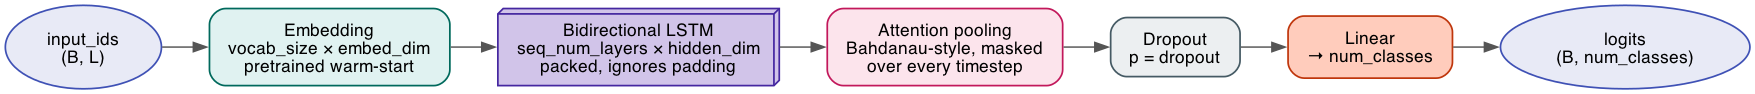
\includegraphics[width=0.9\textwidth]{bilstm_diagram.png}
\caption{BiLSTMClassifier architecture}
\end{figure}

Two omissions are deliberate, not oversights: \texttt{max\_grad\_norm} (gradient-clipping threshold) is
fixed by CLI/config default rather than tuned --- it's a stability safeguard, not an accuracy
lever, so putting it in $\Lambda$ would spend trials on a dimension unlikely to move the metric.
And unlike \texttt{transformer}, there is no \texttt{freeze\_ratio}-equivalent knob: nothing is pretrained
end-to-end here to freeze in the first place, only the embedding matrix, and that is warm-started
rather than frozen.

\section*{Code Flow}

Putting the pieces from the previous sections together, this is what a full search actually
does end to end, from an empty candidate pool to a finished submission.

\begin{figure}[htbp]
\centering
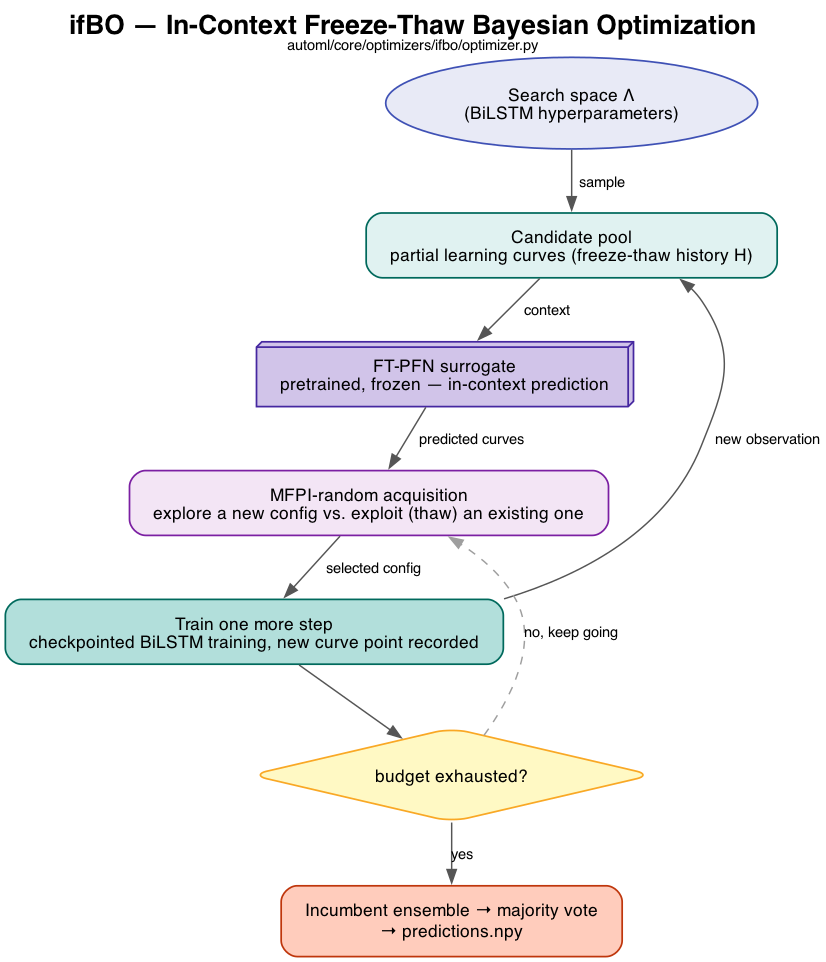
\includegraphics[width=0.9\textwidth]{ifbo_diagram.png}
\caption{The ifBO search loop}
\end{figure}

The search starts with nothing: no configuration has been tried yet, and the candidate pool
is empty. Every iteration opens with a single weighted coin flip that decides whether that
step explores or exploits --- the odds start out heavily favoring exploration, since with an
empty pool there is nothing yet worth exploiting, and gradually shift toward exploitation as
the run progresses and a real pool of partially-trained candidates builds up.

An \textbf{exploration} step is the simple branch: a brand-new configuration is drawn at random
from the search space, dropped straight into the pool, and trained for one step immediately ---
no model, no scoring, no comparison against anything else.

An \textbf{exploitation} step is where the surrogate does its work. Every candidate already in the
pool that hasn't yet been trained to the maximum allowed budget is treated as a contender,
current best-so-far included. All of them are laid before the surrogate model at once,
alongside the complete history of every partial learning curve observed anywhere in the search
so far. The surrogate --- a model trained once, in advance, and never updated again during the
search itself --- reads that history and, for each contender, predicts how likely it is to
cross a target performance level within some number of additional training steps. Neither the
target nor the horizon is fixed: both are redrawn at random on every single round, so the
search never commits to one fixed idea of ``how much better'' or ``how far ahead,'' and instead
samples from a broad spread of possible answers each time. Whichever contender comes out on top
is the one trained further. If there are no contenders at all this round (every pending
candidate is maxed out), a brand-new configuration is sampled instead, the same as an
exploration step.

Whichever branch fires, the chosen configuration is then trained for exactly one more
increment, its progress is checkpointed, and the new point on its learning curve is appended
to the shared history the surrogate will read on the next round. This one-step-at-a-time
cycle --- decide, maybe consult the surrogate, train a little further, record the result ---
repeats until the overall budget of decisions runs out.

At the end of the run, rather than keeping only the single best configuration ever seen, the
strongest handful found across the whole search are retrained to completion and combined by
majority vote, and it is that ensemble's predictions that make up the final submission.

\section*{Results}

Budget:

\begin{verbatim}
max_budget: 10
min_budget: 3
n_trials: 20
\end{verbatim}

\subsection*{Baselines}

Three baselines, each isolating a different piece of what makes the flagship method work ---
every one answers a specific ``would doing less still work?'' question rather than just being an
arbitrary point of comparison:

\begin{itemize}
    \item \textbf{Random Search} --- no multi-fidelity behavior at all: every trial
    samples a fresh configuration uniformly from $\Lambda$ and trains it straight through to
    \texttt{max\_budget} epochs before it's ever compared against anything else. It never resumes a
    partially-trained config and never cuts a bad one short. This is the floor every other method
    has to beat to justify its extra machinery, and it also sets an upper bound on wall-clock cost
    per trial, since it always pays for the \emph{full} epoch budget regardless of how a config is
    doing partway through (see the wall-clock comparison below --- this is exactly why its bars are
    tallest everywhere).
    \item \textbf{SMAC (BO+HB)} --- SMAC3's random-forest-surrogate Bayesian
    optimization, paired with a Hyperband intensifier for multi-fidelity scheduling (successive
    halving: only the top fraction of configs at each rung's budget get promoted to the next,
    larger one). This isolates what a \emph{classical, non-neural} multi-fidelity method achieves under
    the same epoch-budget range as ifBO --- the fairest like-for-like comparison against the
    flagship method, since both get to allocate budget adaptively instead of uniformly, but SMAC
    does it with a random-forest-EI surrogate and a handful of \emph{discrete} Hyperband rungs, instead
    of FT-PFN's in-context transformer and \emph{continuous} freeze-thaw (visible directly in the
    fidelity-allocation figure below: SMAC's budget trace is a coarse two-level sawtooth, ifBO's
    is a much finer staircase).
    \item \textbf{ifBO (random selection)} --- runs the \emph{exact same} freeze-thaw pipeline and candidate-pool
    machinery as the flagship method, but with \texttt{ifbo\_use\_random\_selection=True}: FT-PFN's MFPI-random scoring is swapped for a uniform random choice among that round's pending pool. This is the
    most targeted ablation of the three --- everything about \emph{how much} budget is spent
    incrementally vs.\ upfront is held identical to the flagship run, so any gap between this and
    full ifBO isolates the value of the \emph{surrogate's guidance specifically}, separate from the
    value of freeze-thaw scheduling in general.
\end{itemize}

\textit{Note on the numbers below:} the four runs backing this subsection
(\texttt{sample-results/all\_results/}, timestamped 2026-07-31) predate the removal of the
incumbent-exclusion rule and fresh-candidate-in-exploitation injection described in ``Growing
the candidate pool'' above --- i.e.\ the \texttt{ifBO} column reflects the \emph{earlier}
candidate-selection logic, not the one currently in the codebase. The qualitative story
(freeze-thaw beats fixed-budget search, and surrogate guidance beats random thawing on most
datasets) is expected to hold under the current logic too, but the exact margins below should
not be read as reproducible with today's code without a rerun.

\subsection*{Testbed Results}

All four methods were run under the matched budget above (\texttt{n\_trials=20},
\texttt{min\_budget=3}, \texttt{max\_budget=10} epochs, \texttt{sequence-dl}/BiLSTM search space)
across all five datasets --- \texttt{ag\_news}, \texttt{amazon}, \texttt{dbpedia}, \texttt{imdb}, and the
held-out exam set \texttt{yelp}. Numbers are \textbf{best validation accuracy}
($1 - \min(\text{val\_error})$ over the run), i.e.\ search quality rather than a held-out test
score. Raw histories live in \texttt{sample-results/all\_results}; the figures below are
regenerated straight from those \texttt{.jsonl} files by
\texttt{final\_results\_analysis.ipynb} in that same directory.

\subsubsection*{Final best validation accuracy}

\begin{table}[H]
\centering
\begin{tabular}{@{}lcccc@{}}
\toprule
\textbf{Dataset} & \textbf{ifBO} & \textbf{SMAC (BO+HB)} & \textbf{Random Search} & \textbf{ifBO (random selection)} \\
\midrule
AG News  & 91.35\% & 89.35\% & 89.65\% & \textbf{92.45\%} \\
Amazon   & \textbf{89.15\%} & 78.20\% & 79.25\% & 79.30\% \\
DBpedia  & \textbf{97.85\%} & 97.00\% & 97.80\% & 97.70\% \\
IMDB     & \textbf{93.80\%} & 85.25\% & 86.70\% & 87.70\% \\
Yelp     & \textbf{58.10\%} & 50.50\% & 55.10\% & 54.35\% \\
\bottomrule
\end{tabular}
\caption{Best validation accuracy per dataset and method.}
\end{table}

Full ifBO (FT-PFN-guided) wins on 4 of 5 datasets, with the largest margins on the hardest
tasks --- Amazon (+9.90pp over the best baseline) and Yelp (+3.0pp over Random, +7.6pp over
SMAC). On AG News, its own random-selection ablation edges it out (92.45\% vs.\ 91.35\%) --- on
the easiest dataset in the suite (all four methods clear 89\%), the FT-PFN surrogate's
acquisition doesn't have much signal to exploit over unguided freeze-thaw scheduling, so the two
land within noise of each other. Everywhere else, guided candidate selection is what separates
ifBO from its own ablation.

\begin{figure}[H]
\centering
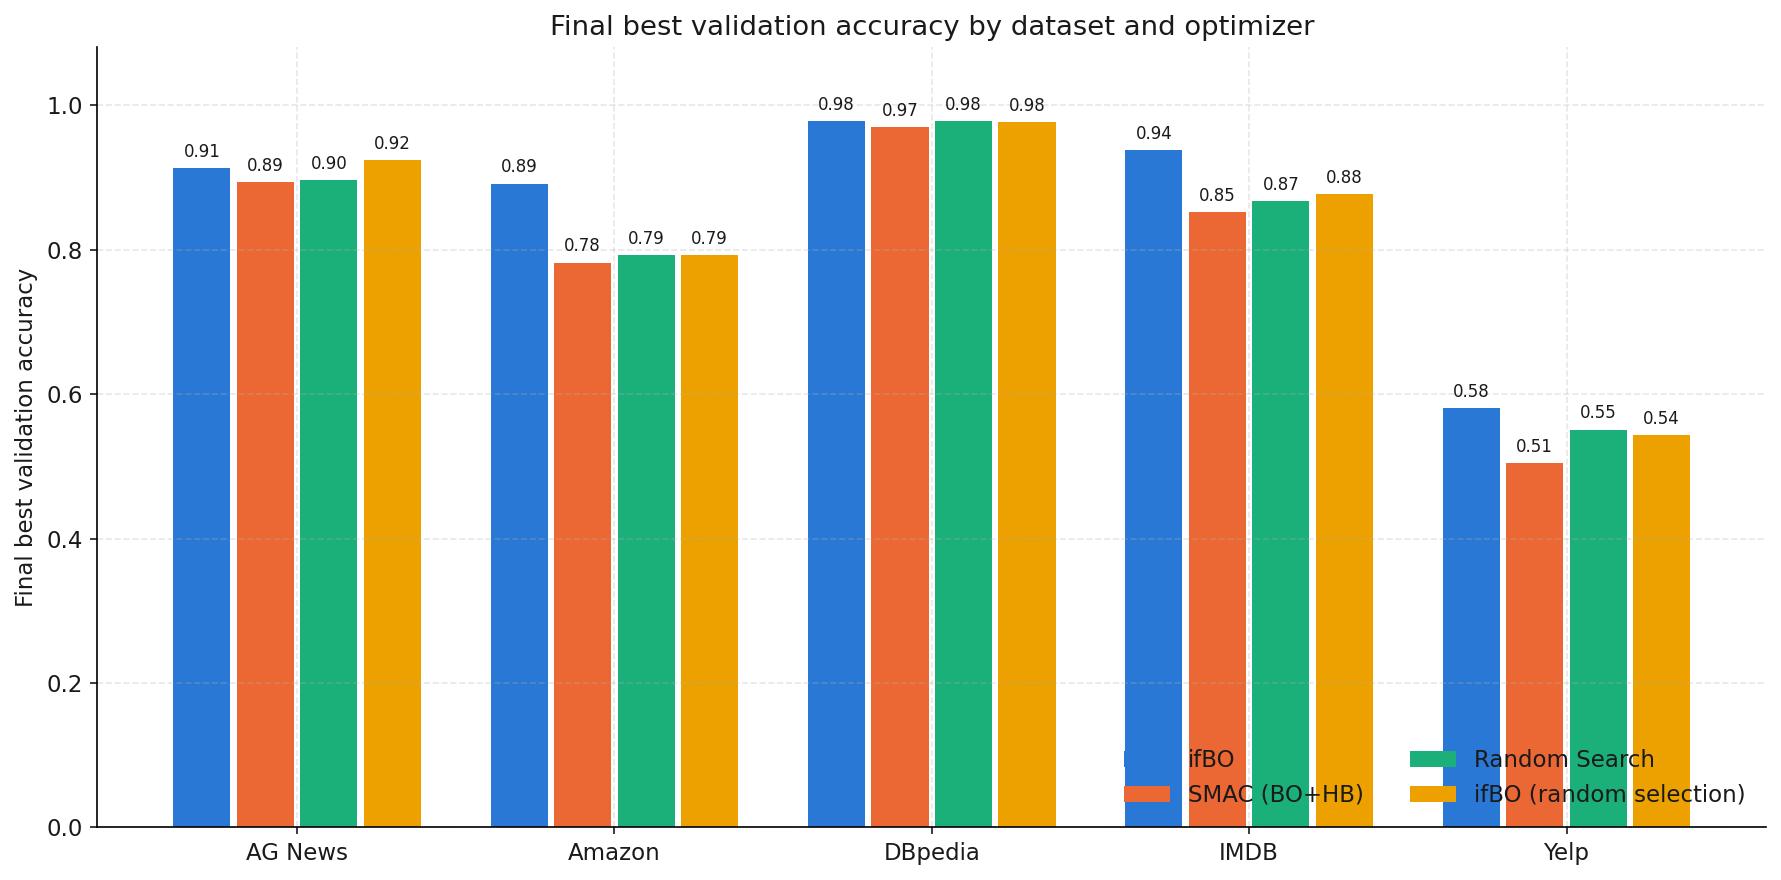
\includegraphics[width=0.85\textwidth]{figures/03_final_accuracy_bars.png}
\caption{Final accuracy bars per dataset and method.}
\end{figure}

The bar chart above puts all four methods side by side per dataset --- read it for
\emph{magnitude} of the gaps (Amazon and Yelp show real daylight between ifBO and everything
else; AG News and DBpedia show all four methods bunched within a couple of points). The heatmap
below is the same numbers, but its shading makes the two structurally different
failure/success stories in this table pop out immediately: DBpedia's whole row is uniformly
dark (97--98\% for \emph{every} method) --- with \texttt{max\_budget=10} epochs, this dataset is close
to saturated for the \texttt{sequence-dl} search space, so there's little room for any optimizer to
differentiate itself. Yelp's row is uniformly the lightest (50--58\%) --- every method tops out
well below where it lands on the other four datasets, so Yelp is a genuinely harder
classification problem at this fidelity budget, not just a dataset where the optimizer happened
to do badly.

\begin{figure}[H]
\centering
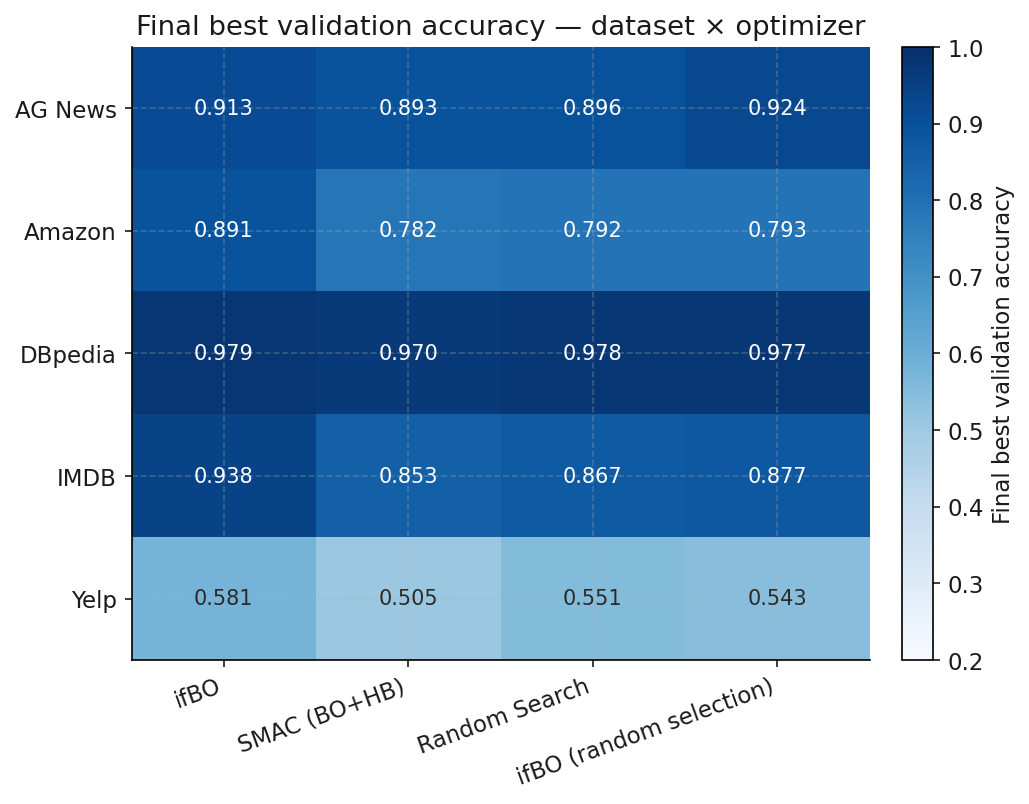
\includegraphics[width=0.75\textwidth]{figures/04_accuracy_heatmap.png}
\caption{Accuracy heatmap across datasets and methods.}
\end{figure}

\subsubsection*{Sample efficiency and wall-clock cost}

Freeze-thaw's structural advantage shows up earliest here: both ifBO variants pull ahead of
Random/SMAC within the first several trials on every dataset, because a handful of thaw steps
into one promising candidate teach the surrogate (or even just the epsilon-floor exploration
alone) more than one epoch each spent across many never-revisited configs. The step lines below
are the running best-so-far incumbent; faint dots are every individual trial actually sampled,
so the vertical spread of dots at a given x tells you how much the optimizer is still gambling on
long shots even after it's found something good. SMAC's characteristic pattern is a late, sharp
jump once a Hyperband rung promotes a strong config --- it's blind to that config's promise until
the rung boundary says to check on it again (its budget trace only ever touches two values,
$\sim$3.3 and 10 epochs, see the fidelity-allocation figure below), unlike ifBO's much smoother,
earlier climb.

\begin{figure}[H]
\centering
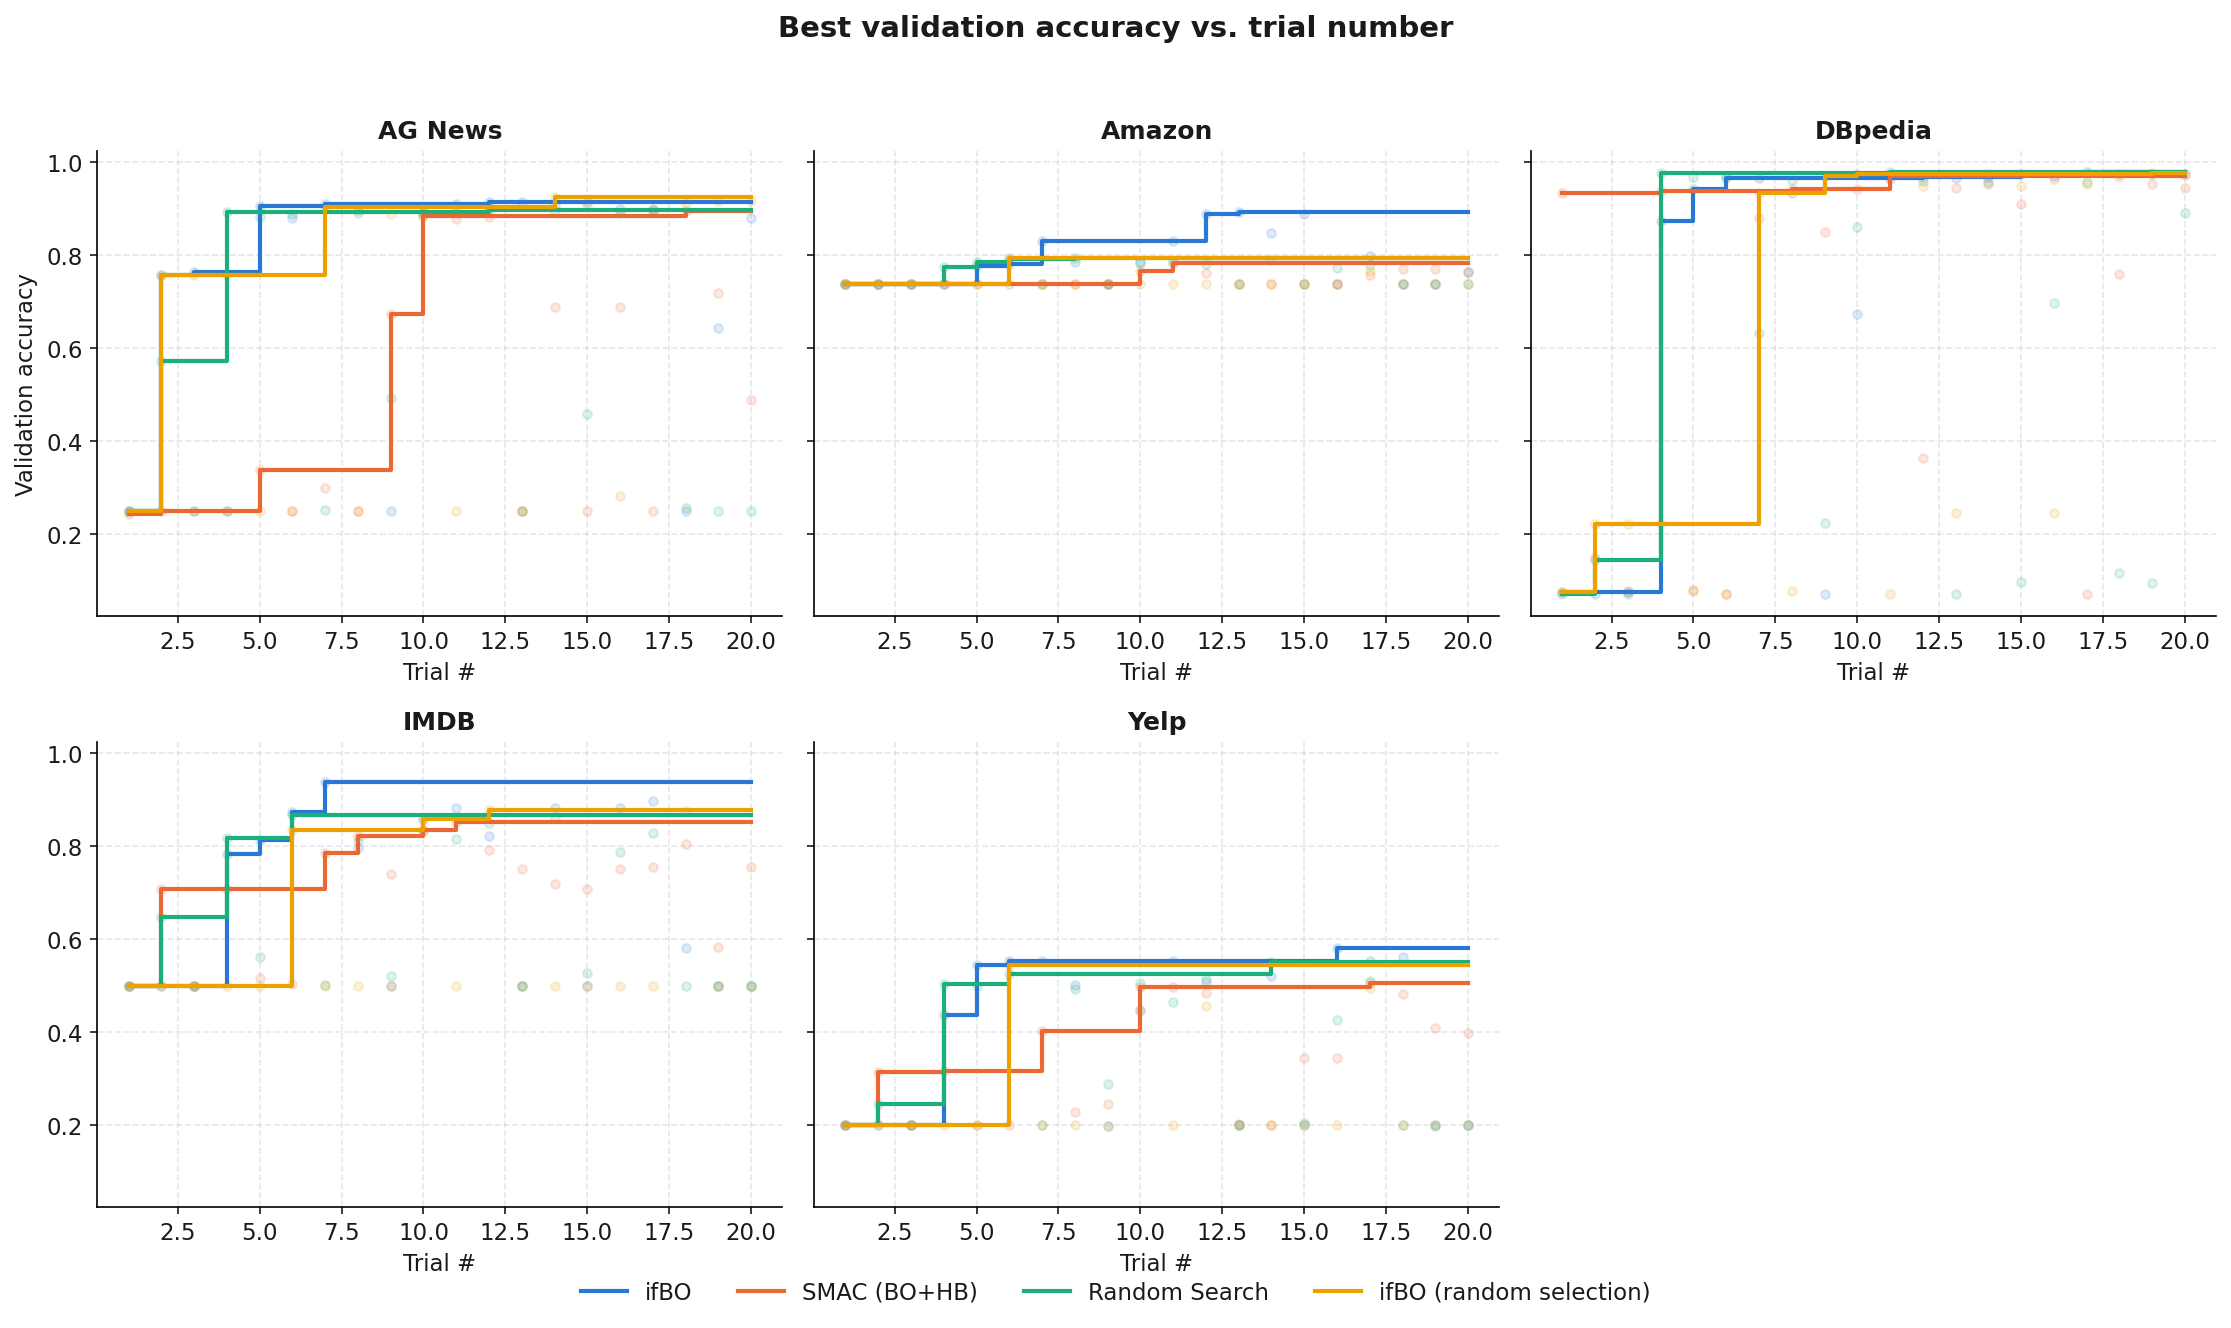
\includegraphics[width=0.9\textwidth]{figures/02_best_vs_trial.png}
\caption{Best validation accuracy vs.\ trial number.}
\end{figure}

Against wall-clock time, the same curves stretch out very differently per method: Random
Search's step lines are still moving well after both ifBO variants have converged and gone
flat, since every single trial (good or bad) costs it a full \texttt{max\_budget}-epoch training
run --- it simply hasn't finished sampling yet by the time freeze-thaw has already plateaued.

\begin{figure}[H]
\centering
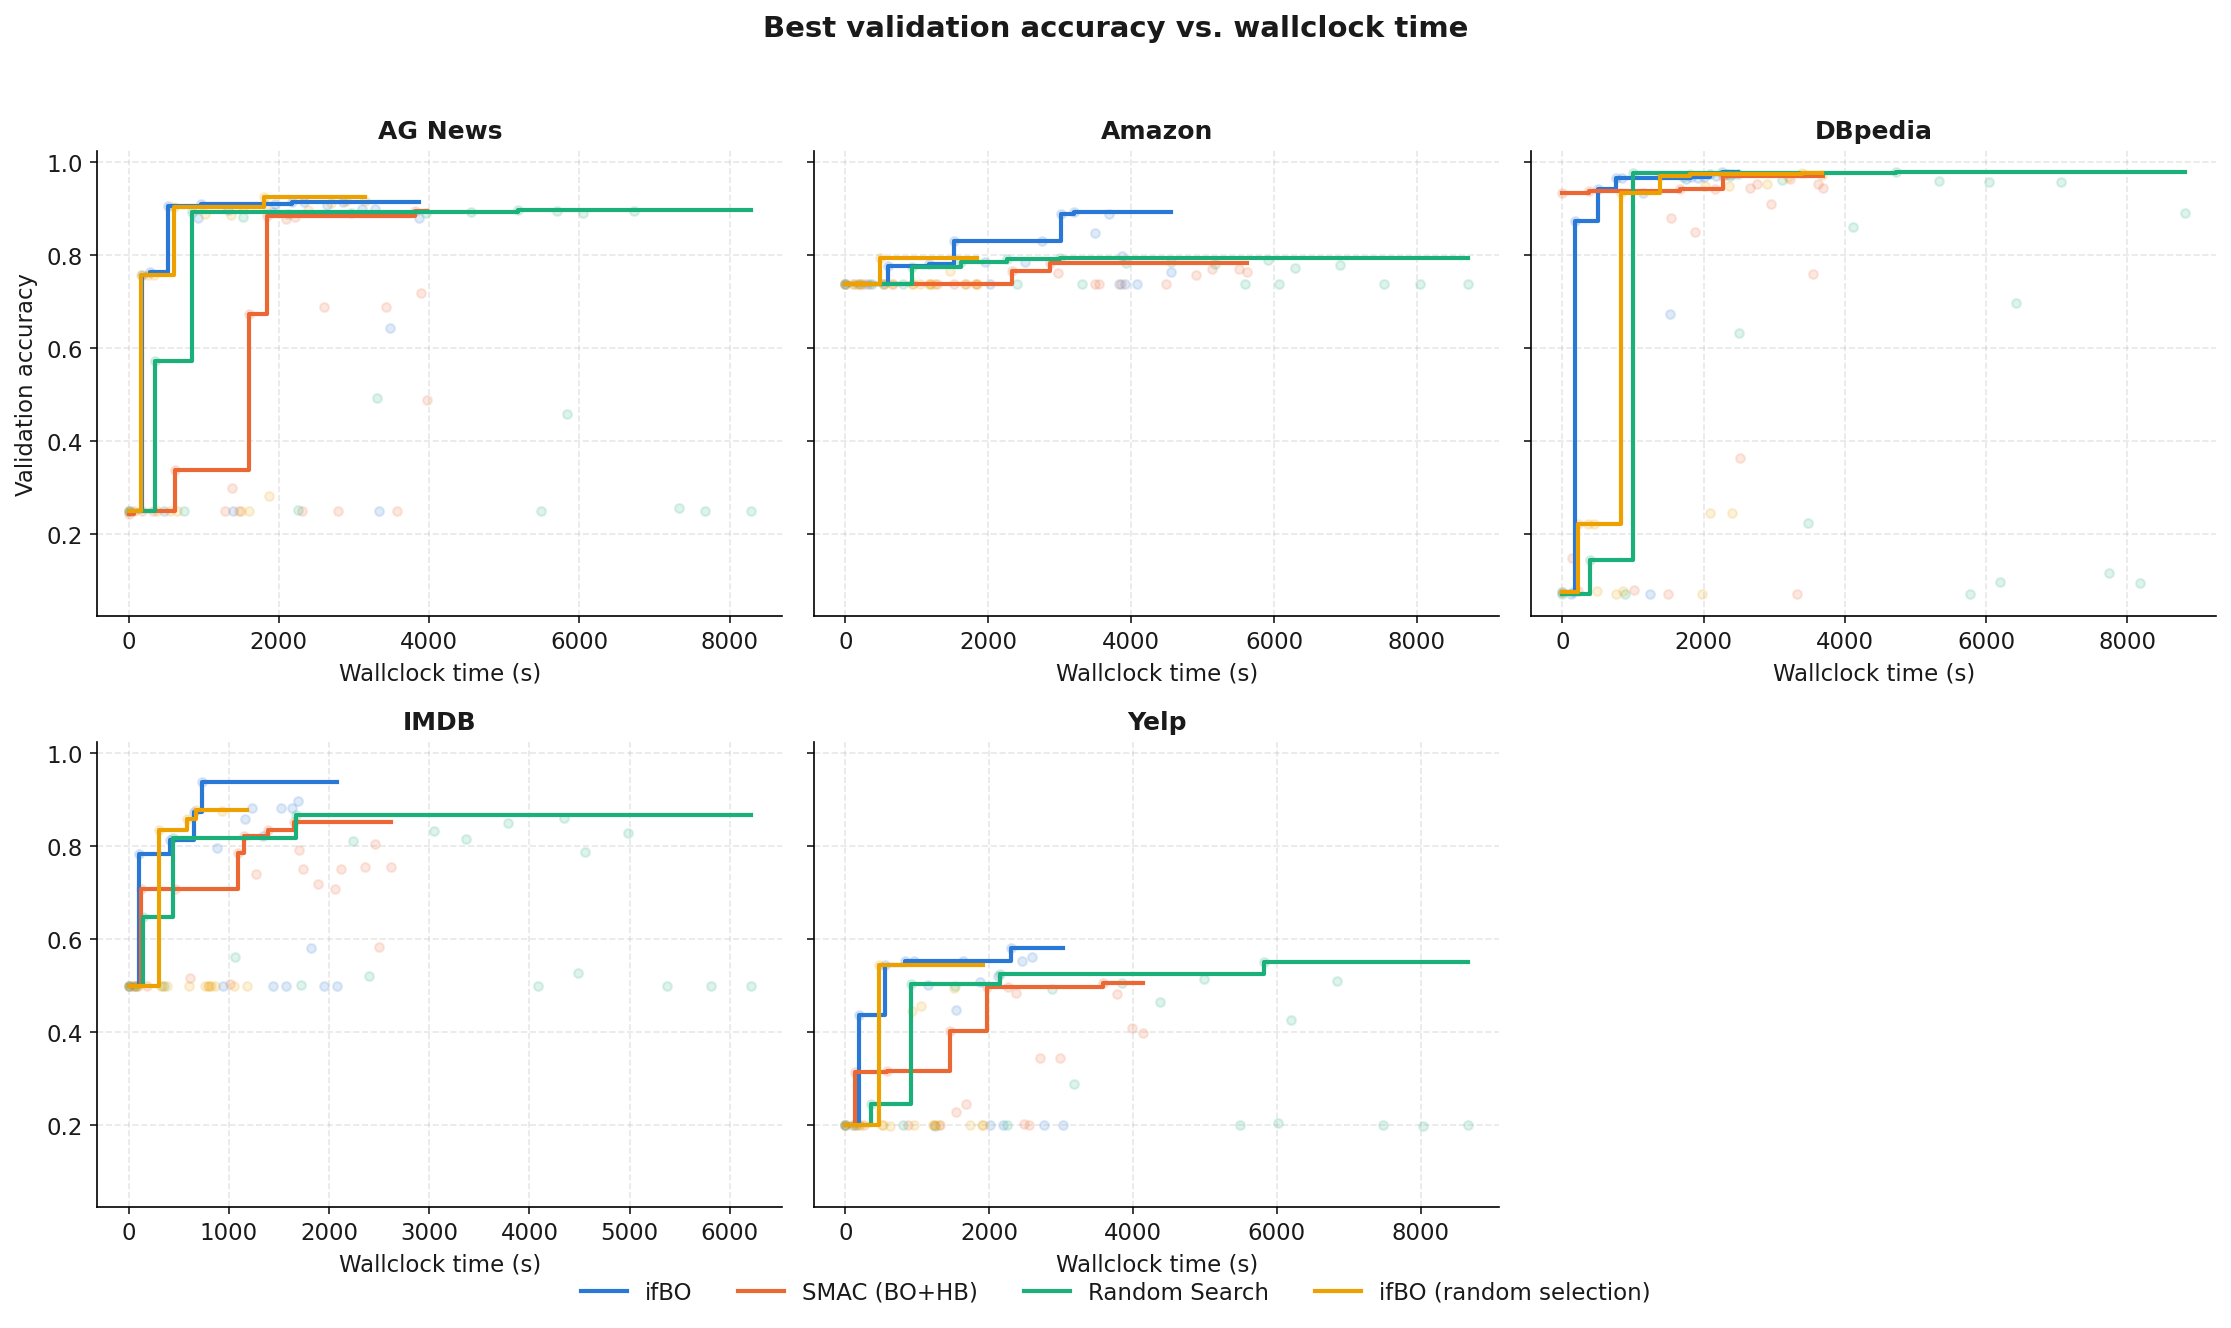
\includegraphics[width=0.9\textwidth]{figures/01_best_vs_wallclock.png}
\caption{Best validation accuracy vs.\ wall-clock time.}
\end{figure}

Total wall-clock (elapsed time from the first trial's start to the last trial's start, over all
20 trials of a run) tells the same story in aggregate: Random Search consistently takes
2--4$\times$ longer than either ifBO variant for a 20-trial run (e.g.\ $\sim$147 vs.\ $\sim$41
minutes on DBpedia, $\sim$144 vs.\ $\sim$50 on Yelp), without a corresponding accuracy payoff. A
subtler gap sits between the two ifBO variants themselves: the random-selection ablation is
consistently faster than the full surrogate-guided run on every dataset (e.g.\ $\sim$31 vs.\
$\sim$76 minutes on Amazon, $\sim$20 vs.\ $\sim$35 on IMDB) despite following an identical
freeze-thaw training schedule --- the difference is pure FT-PFN inference overhead, one batched
forward pass through the surrogate on every exploitation round, which the ablation skips
entirely by picking uniformly at random instead.

\begin{figure}[H]
\centering
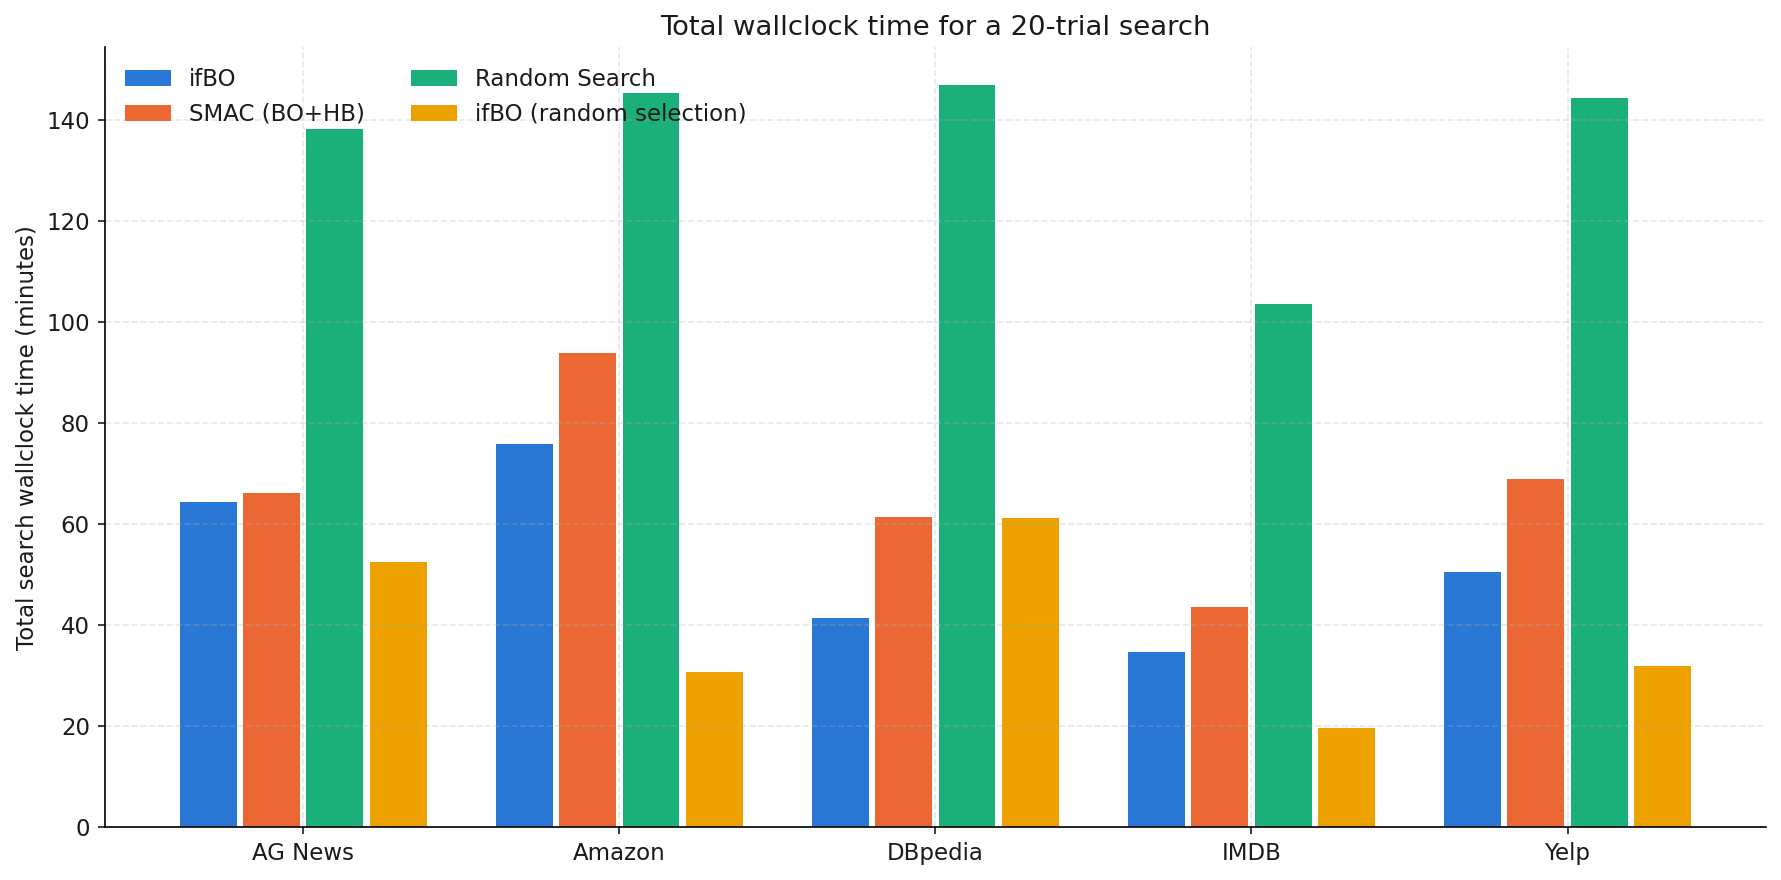
\includegraphics[width=0.85\textwidth]{figures/08_total_wallclock.png}
\caption{Total wall-clock time per dataset and method.}
\end{figure}

\subsubsection*{Where the budget goes}

The per-trial accuracy distribution below shows \emph{every} sampled trial, not just the
incumbent --- a tighter, higher box means an optimizer is spending steps on consistently good
configs rather than wasting them on poor ones. ifBO's box is the tightest and highest of the
four on most datasets, direct evidence that surrogate-guided selection is concentrating repeat
thaws on configs already known to be good rather than spending them on fresh gambles. Random's
and SMAC's boxes are consistently the widest, spanning from floor accuracy up to their max ---
both are still spending real trials on poor draws this late into the search, since neither can
\texttt{thaw}-revisit a specific promising config on demand the way freeze-thaw can.

\begin{figure}[H]
\centering
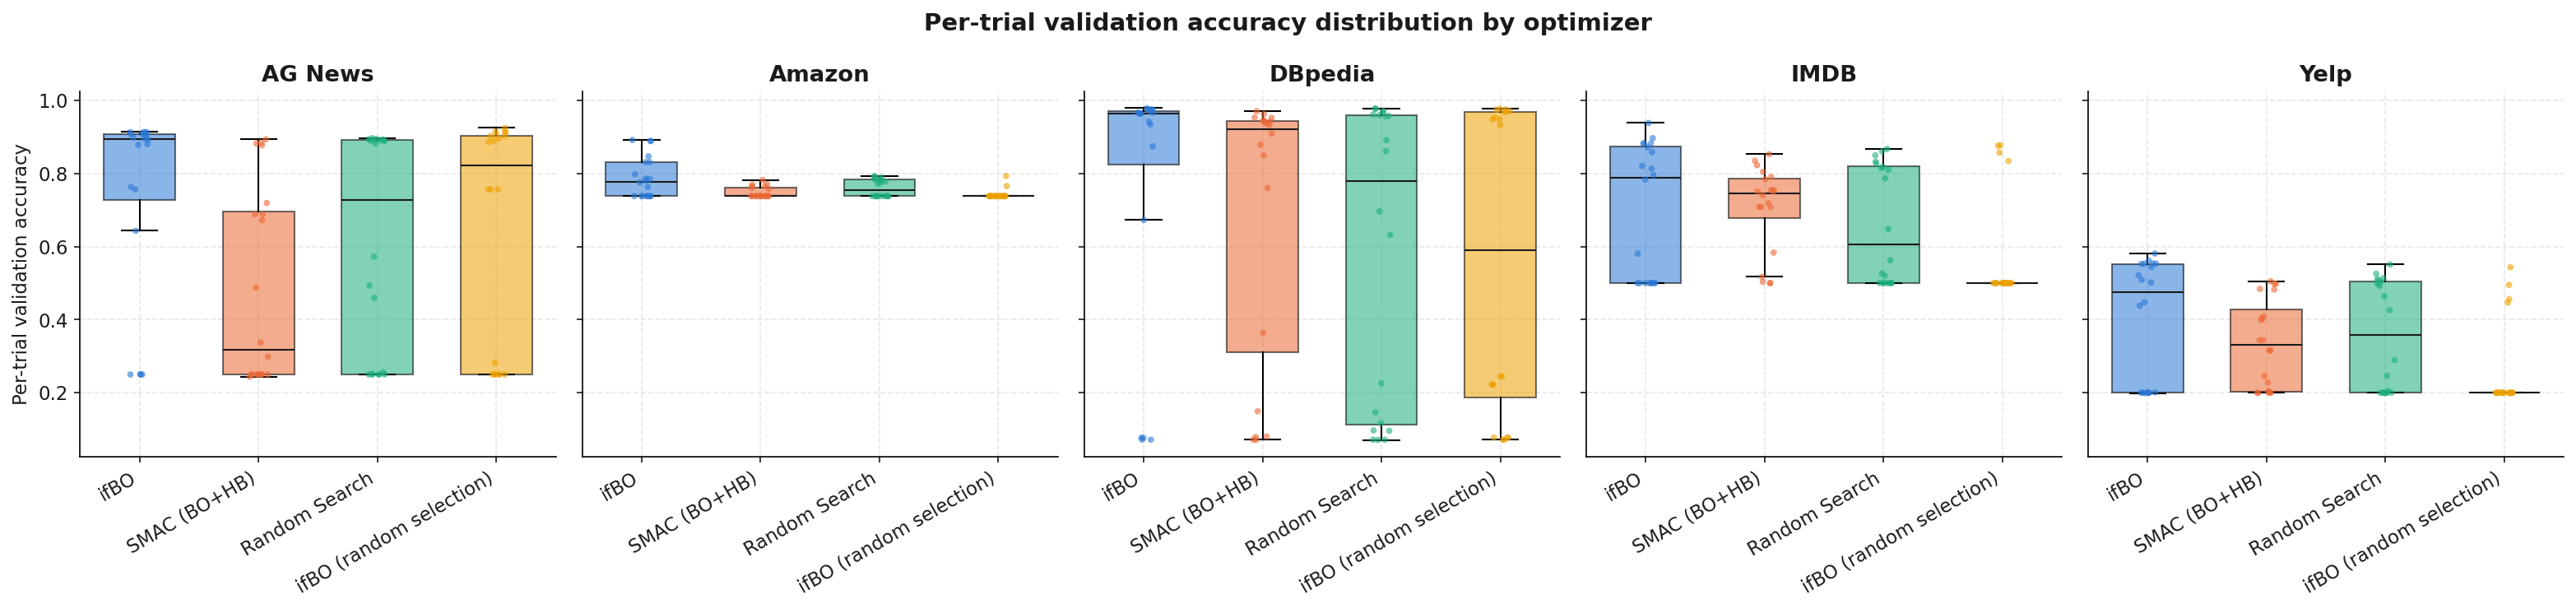
\includegraphics[width=0.9\textwidth]{figures/05_accuracy_boxplots.png}
\caption{Per-trial accuracy distribution.}
\end{figure}

The epoch-budget plot makes the \emph{shape} of each method's multi-fidelity policy visible
directly, trial by trial. Random Search is a flat ceiling line at \texttt{max\_budget} by
construction --- it has no multi-fidelity policy. SMAC's Hyperband intensifier produces a coarse,
almost binary sawtooth that only ever touches two values ($\sim$3.3 and 10 epochs) --- at this
budget range the successive-halving bracket only has two rungs, so a config is either killed at
the bottom rung or promoted straight to the top one, with nothing in between. Both ifBO variants
instead walk the \emph{entire} epoch grid (4, 5, 6, 7, 8, 9, \ldots) --- the direct visual signature
of literal one-step-at-a-time freeze-thaw: a config is thawed for one more increment,
re-evaluated, and only then is the next decision made, rather than being judged at a small
number of fixed checkpoints.

\begin{figure}[H]
\centering
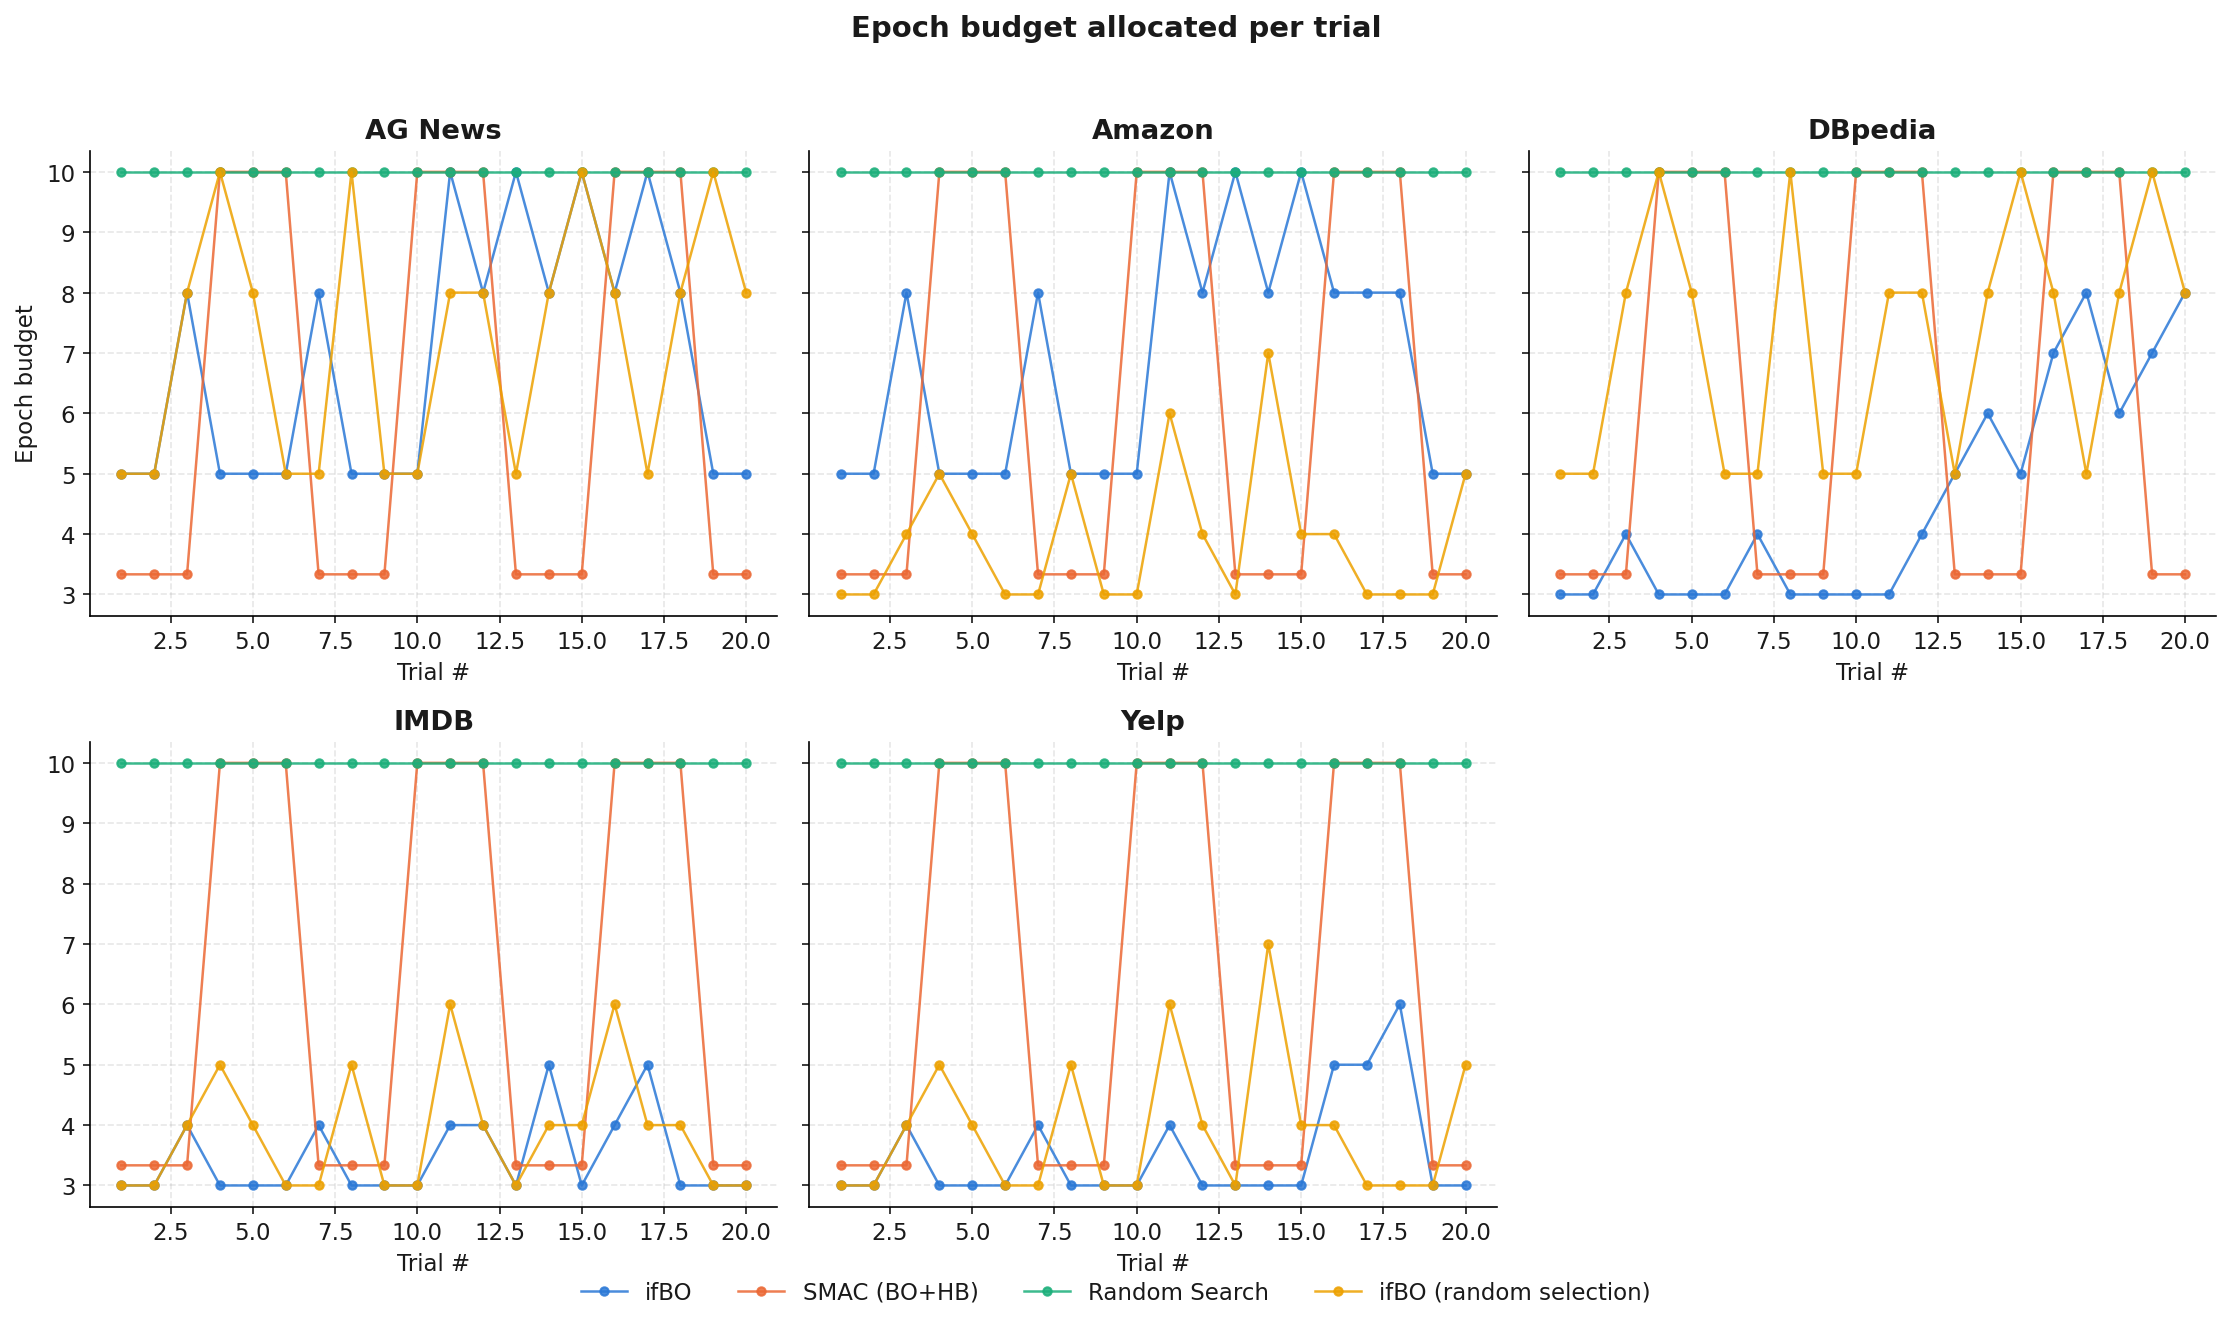
\includegraphics[width=0.9\textwidth]{figures/06_fidelity_allocation.png}
\caption{Epoch budget allocated per trial.}
\end{figure}

Finally, the training curve of each method's single best-found configuration per dataset ---
this is the one figure that shows \emph{within-run} learning-curve shape rather than
across-trial search behavior. On IMDB, ifBO's best config reaches 93.8\% accuracy in just 4
epochs and its curve stops there (that's all the budget it was ever thawed for), while SMAC's
best config needs the full 10 epochs to climb to only 85.25\% --- a smaller number reached with
more than double the training cost, since freeze-thaw was able to recognize this config's
quality early and never needed to push it further.

\begin{figure}[H]
\centering
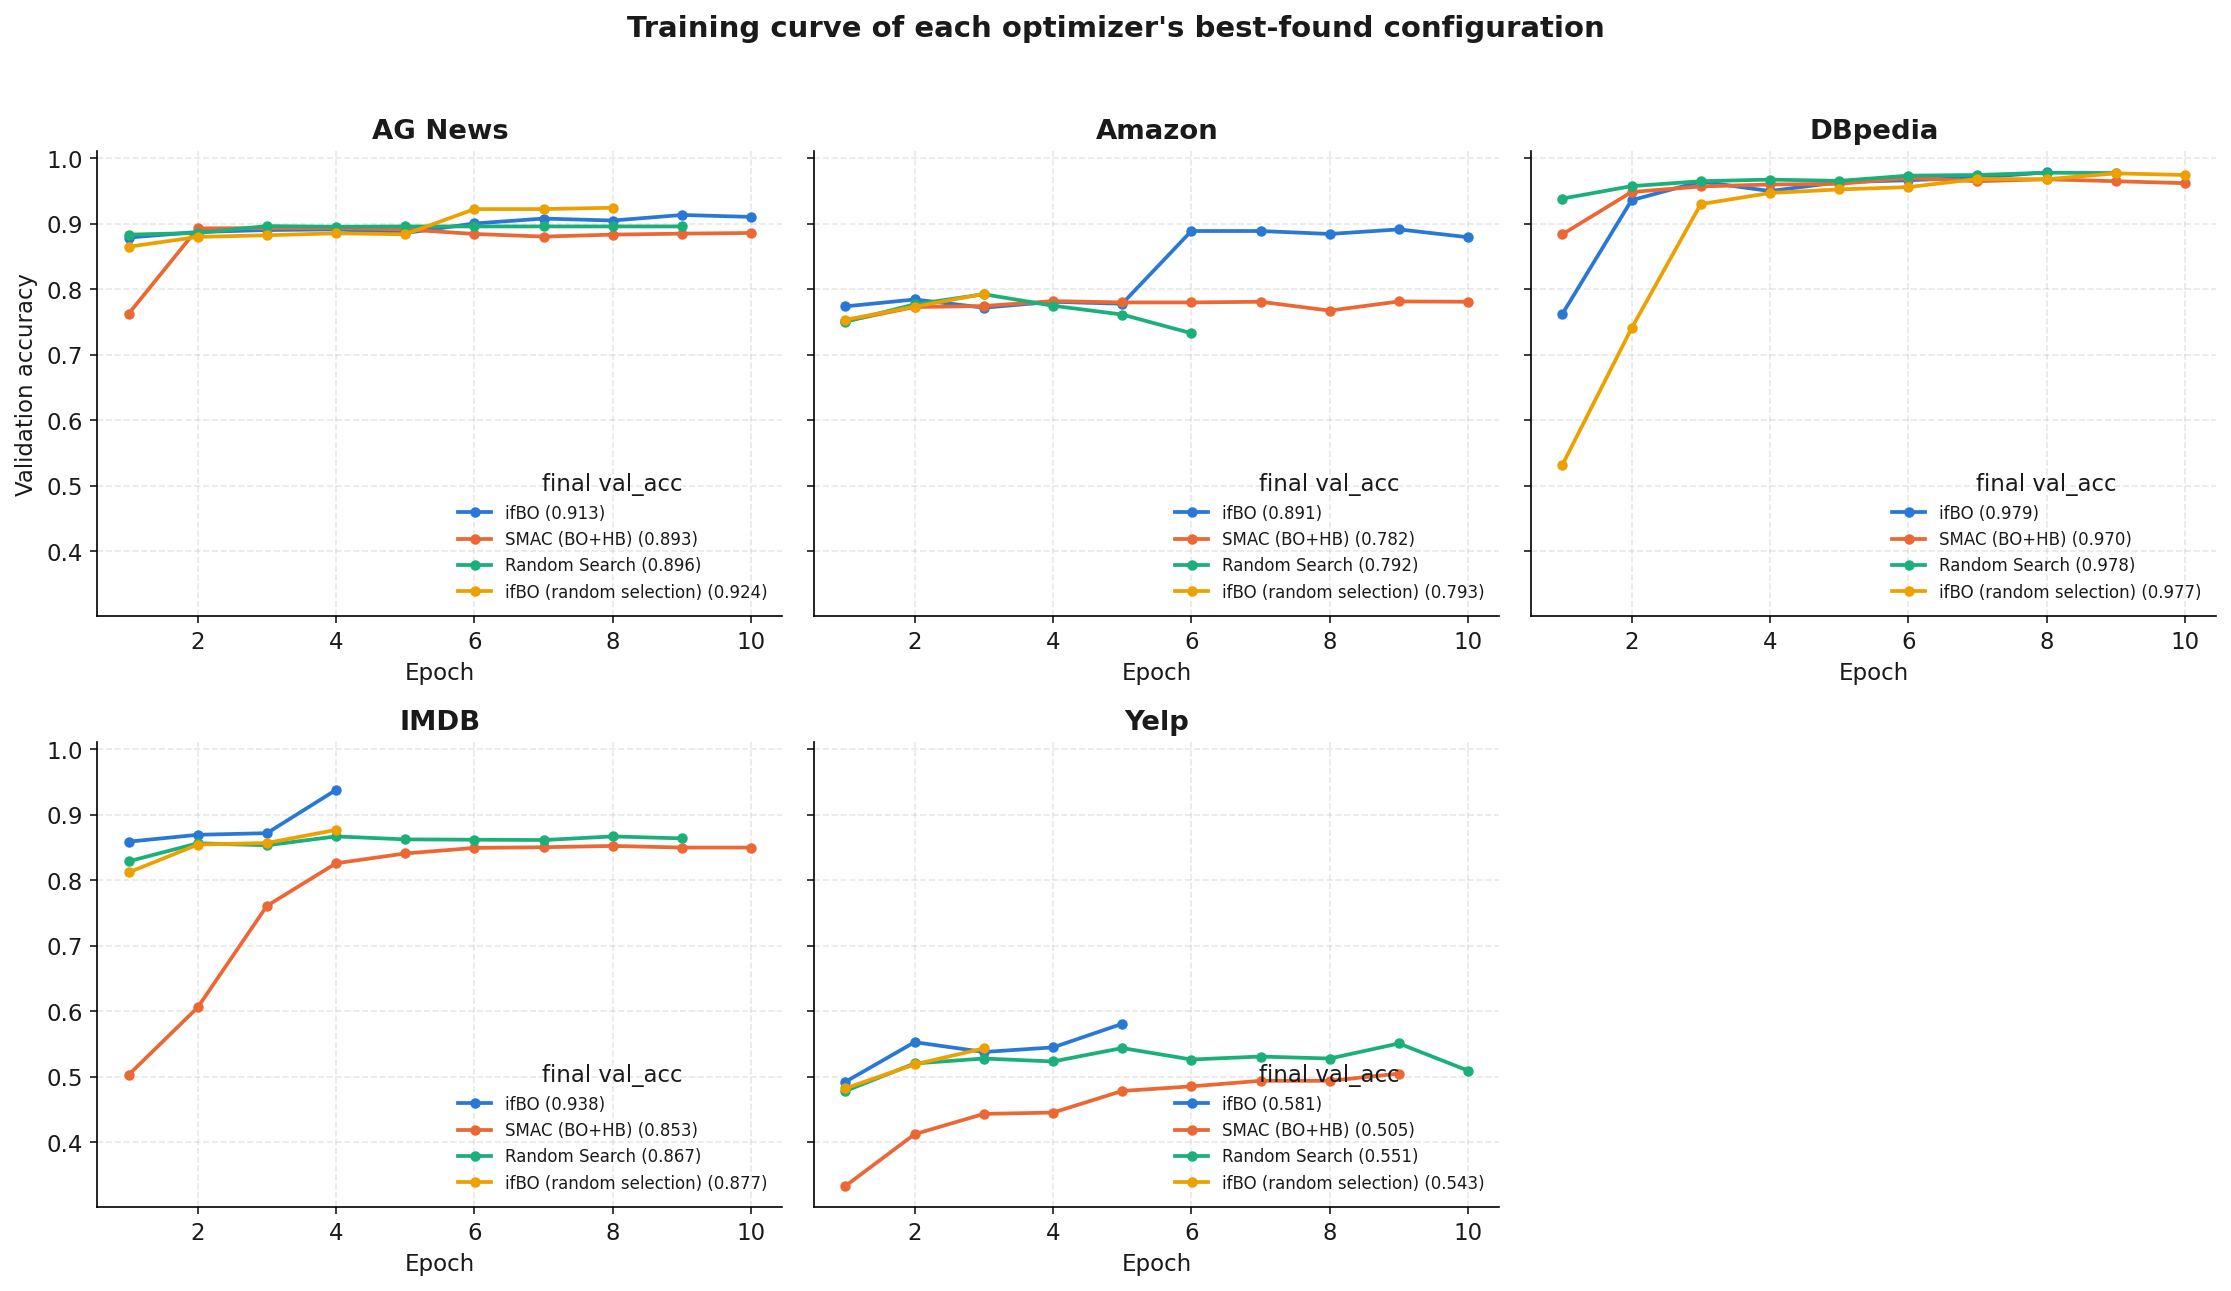
\includegraphics[width=0.9\textwidth]{figures/07_best_trial_curves.png}
\caption{Best trial training curves per dataset.}
\end{figure}

\subsection*{Final Submission Results}

\begin{center}
\begin{tabular}{lccc}
\hline
Dataset & Test Accuracy & Reference Accuracy & $\Delta$ vs.\ Reference \\
\hline
AG News & 91.27\% & 90.265\% & 1.005\% \\
Amazon & 82.33\% & 81.799\% & +0.53\% \\
DBpedia & 98.77\% & 97.882\% & +0.888\% \\
IMDB & 84.16\% & 86.993\% & -2.83\% \\
Yelp & 64.35\% & 62.082\% & +2.268\% \\
\hline
\end{tabular}
\end{center}

\end{document}